\documentclass[10pt]{article}

% Packages
\usepackage{booktabs}
\usepackage{graphicx}
\usepackage{amsmath}
\usepackage{geometry}
\usepackage{pgfplots}
\usepackage{pgfplotstable}
\pgfplotsset{compat=1.18}
\geometry{margin=1in}

\title{Evaluation of CosPlace and LoFTR-Based Reranking for Visual Place Recognition}
\author{}
\date{}

\begin{document}

\maketitle

% ---------------------------------------------------------
% TABLE
% ---------------------------------------------------------
\begin{table}[t]
\centering
\caption{Top-1 accuracy (\%) and reranking time (minutes) for CosPlace (baseline), CosPlace+LoFTR Adaptive Reranking, and CosPlace+LoFTR Full Reranking across four VPR benchmarks.}
\label{tab:adaptive_vs_full}

\resizebox{\linewidth}{!}{
\begin{tabular}{lcccc}
\toprule
\textbf{Dataset} & \textbf{CosPlace} & \textbf{Adaptive (CosPlace+LoFTR)} & \textbf{Full (CosPlace+LoFTR)} & \textbf{Time (A / F)} \\
\midrule
SF-XS-test       & 70.0 & 78.0 & \textbf{81.3} & 10 / 39 \\
SVOX-test-sun    & 73.0 & 87.0 & \textbf{90.1} & 9 / 32 \\
SVOX-test-night  & 49.0 & 72.0 & \textbf{73.5} & 17 / 31 \\
Tokyo-test       & 70.0 & 84.0 & \textbf{85.7} & 4 / 12 \\
\bottomrule
\end{tabular}
}
\end{table}

% ---------------------------------------------------------
% ACCURACY BAR CHART
% ---------------------------------------------------------
\section{Top-1 Accuracy Comparison}

\begin{figure}[h!]
\centering
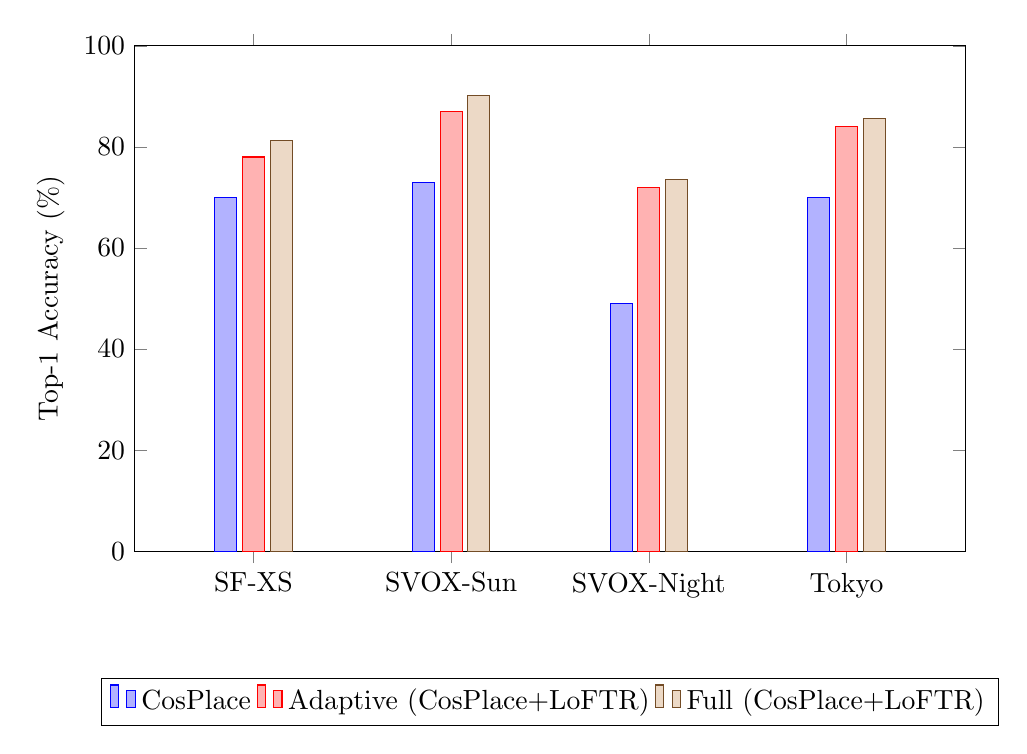
\begin{tikzpicture}
\begin{axis}[
    ybar,
    bar width=8pt,
    width=\linewidth,
    height=8cm,
    enlarge x limits=0.2,
    ylabel={Top-1 Accuracy (\%)},
    symbolic x coords={SF-XS,SVOX-Sun,SVOX-Night,Tokyo},
    xtick=data,
    legend style={at={(0.5,-0.25)},anchor=north,legend columns=3},
    ymin=0, ymax=100
]

\addplot coordinates {(SF-XS,70) (SVOX-Sun,73) (SVOX-Night,49) (Tokyo,70)};
\addplot coordinates {(SF-XS,78) (SVOX-Sun,87) (SVOX-Night,72) (Tokyo,84)};
\addplot coordinates {(SF-XS,81.3) (SVOX-Sun,90.1) (SVOX-Night,73.5) (Tokyo,85.7)};

\legend{CosPlace, Adaptive (CosPlace+LoFTR), Full (CosPlace+LoFTR)}
\end{axis}
\end{tikzpicture}
\caption{Top-1 accuracy of the three evaluated methods across all benchmarks.}
\end{figure}

% ---------------------------------------------------------
% TOP-1 ACCURACY SECTION
% ---------------------------------------------------------
\section{Top-1 Accuracy}

This experiment compares three setups:

\begin{itemize}
    \item \textbf{CosPlace}: descriptor-only baseline.
    \item \textbf{CosPlace + LoFTR (Adaptive Reranking)}: LoFTR is applied only to a selected subset of candidates.
    \item \textbf{CosPlace + LoFTR (Full Reranking)}: LoFTR is applied to all top candidates.
\end{itemize}

Both reranking strategies improve the baseline on every dataset.

\subsection{Overall Trends}

CosPlace alone gives a solid starting point, but adding LoFTR always increases accuracy.  
Adaptive Reranking gives most of the improvement while keeping the runtime low.  
Full Reranking gives the highest accuracy but is much slower.

The biggest improvements appear on SVOX-test-night, where lighting changes make descriptor-only retrieval difficult.

\subsection{Relative Improvements}

The relative gain of Adaptive Reranking over CosPlace is:

\begin{itemize}
    \item SF-XS-test: 11.4\%
    \item SVOX-test-sun: 19.2\%
    \item SVOX-test-night: 46.9\%
    \item Tokyo-test: 20.0\%
\end{itemize}

\begin{figure}[h!]
\centering
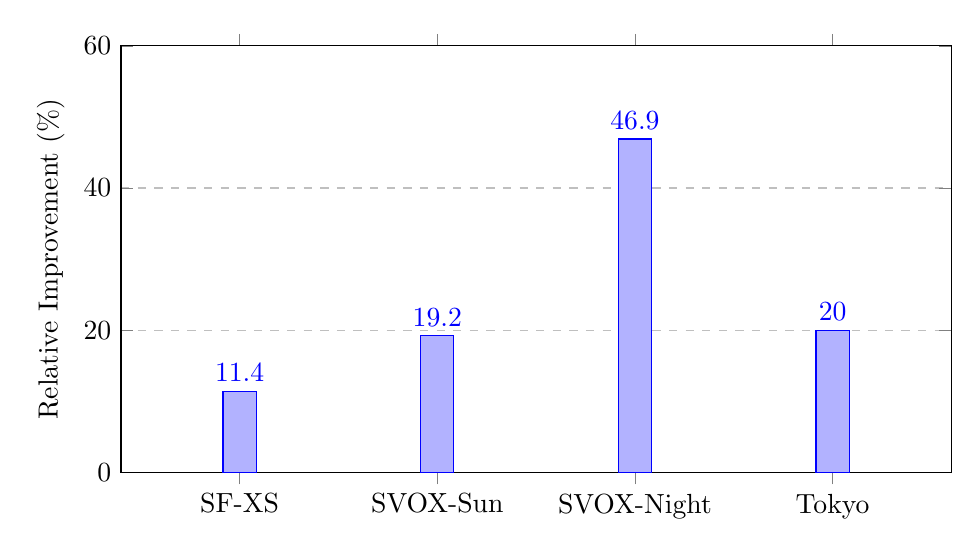
\begin{tikzpicture}
\begin{axis}[
    ybar,
    bar width=12pt,
    width=\linewidth,
    height=7cm,
    enlarge x limits=0.2,
    ylabel={Relative Improvement (\%)},
    symbolic x coords={SF-XS,SVOX-Sun,SVOX-Night,Tokyo},
    xtick=data,
    ymin=0, ymax=60,
    nodes near coords,
    nodes near coords align={vertical},
    ymajorgrids=true,
    grid style=dashed
]

\addplot coordinates {
    (SF-XS,11.4)
    (SVOX-Sun,19.2)
    (SVOX-Night,46.9)
    (Tokyo,20.0)
};

\end{axis}
\end{tikzpicture}
\caption{Relative improvement of Adaptive Reranking over CosPlace across all datasets.}
\end{figure}

Nighttime data shows the strongest improvement, confirming that LoFTR helps when appearance cues are unreliable.



% ---------------------------------------------------------
% RECOVERY RATIO
% ---------------------------------------------------------
\subsection{Recovery Ratio}

Adaptive Reranking recovers most of the accuracy that Full Reranking provides:

\begin{itemize}
    \item SF-XS-test: 73\%
    \item SVOX-test-sun: 80\%
    \item SVOX-test-night: 93\%
    \item Tokyo-test: 88\%
\end{itemize}

\subsection{Dataset Observations}

\begin{itemize}
    \item \textbf{Nighttime sequences}: largest gains, LoFTR helps resolve descriptor failures.
    \item \textbf{Daytime datasets}: strong but smaller improvements.
    \item \textbf{Simpler datasets}: smaller gains, consistent with lower difficulty.
\end{itemize}

% ---------------------------------------------------------
% RUNTIME BAR CHART
% ---------------------------------------------------------
\section{Reranking Runtime Comparison}

\begin{figure}[h!]
\centering
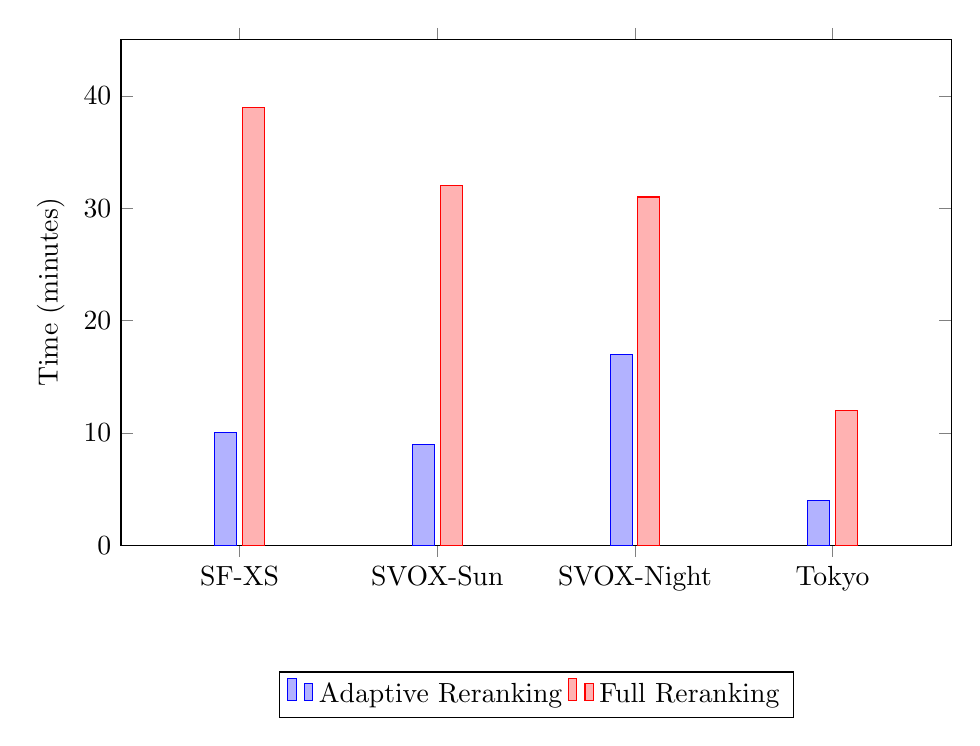
\begin{tikzpicture}
\begin{axis}[
    ybar,
    bar width=8pt,
    width=\linewidth,
    height=8cm,
    enlarge x limits=0.2,
    ylabel={Time (minutes)},
    symbolic x coords={SF-XS,SVOX-Sun,SVOX-Night,Tokyo},
    xtick=data,
    legend style={at={(0.5,-0.25)},anchor=north,legend columns=2},
    ymin=0, ymax=45
]

\addplot coordinates {(SF-XS,10) (SVOX-Sun,9) (SVOX-Night,17) (Tokyo,4)};
\addplot coordinates {(SF-XS,39) (SVOX-Sun,32) (SVOX-Night,31) (Tokyo,12)};

\legend{Adaptive Reranking, Full Reranking}
\end{axis}
\end{tikzpicture}
\caption{Runtime of the two LoFTR-based reranking strategies.}
\end{figure}

% ---------------------------------------------------------
% ANALYSIS SECTION
% ---------------------------------------------------------
\section{Analysis}

The results show a clear trade-off between accuracy and runtime.  
Full Reranking gives the best accuracy but is slow because LoFTR is applied to all candidates.  
Adaptive Reranking is much faster and still recovers most of the accuracy gain.

Across all datasets, the ranking is consistent:

\[
\text{CosPlace} < \text{Adaptive Reranking} < \text{Full Reranking}
\]

This makes the evaluation reliable and easy to extend with more methods in the future.

% ---------------------------------------------------------
% SUMMARY
% ---------------------------------------------------------
\section{Summary}

We evaluated CosPlace, CosPlace+LoFTR Adaptive Reranking, and CosPlace+LoFTR Full Reranking across four benchmarks.  
Both reranking methods improve the baseline, with the largest gains appearing in difficult visual conditions.  
Adaptive Reranking offers a strong balance between accuracy and speed, while Full Reranking provides the highest accuracy at a higher cost.  
This framework can be extended with additional reranking or matching methods in future work.

\end{document}